\documentclass[a4paper,12pt]{article}

\usepackage{geometry}
\geometry{top=15mm}
\geometry{bottom=30mm}
\geometry{left=10mm}
\geometry{right=20mm}
\linespread{1}
\setlength{\parindent}{12pt}
\setlength{\parskip}{8pt}

\usepackage{titleps}

\newpagestyle{main}
{
  \setheadrule{0.4pt}
  \sethead{}{}{}
  \setfootrule{0,4pt}
  \setfoot{}{\thepage}{}
}
\usepackage{color}
\usepackage[english,russian]{babel}
\usepackage[T2A]{fontenc}
\usepackage[utf8]{inputenc}
\usepackage{amsthm,amsmath,amsfonts,amssymb,mathtools}
\usepackage{indentfirst}
\usepackage{lipsum}
\usepackage{graphicx}
\usepackage{float}
\usepackage{wrapfig}

\newcommand{\partdef}[2]{\frac{\partial \mathnormal{#1}}{\partial \mathnormal{#2}}}

\begin{document}

\begin{center}
\textbf{
Численное решение краевой задачи принципа максимума в задаче оптимального управления методом стрельбы.
}
\end{center}





\section{Постановка задачи.}
Рассматривается задача Лагранжа с фиксированным временным отрезком и без ограничений вида "меньше или равно":
\begin{align}
\begin{align*}
    B_0=\int_0^T({\ddot x}^2-{\dot x}^2-x^2)dt
\end{align*}
\end{align}

Требуется формализовать задачу, как задачу оптимального управления. Свести задачу принципом максимума Понтрягина к краевой задаче, численно решить полученную задачу методом стрельбы и обосновать точность полученных результатов. Проверить полученные экстремали Понтрягина на оптимальность при различных значениям параметра $T \in \{0.1,1,10,20\}.$


\section{Формализация задачи.}
Формализуем задачу, как задачу оптимального управления. Для этого обозначим $u= \ddot x, y=\dot x $. Тогда наша задача примет следующий вид:
\begin{align}
\begin{align*}
    \left\{
        \begin{array}{l}
            {\dot x}=y
            \\
            {\dot y}=u
            \\
            u \in \left[-1,1\right]
            \\
            x(0)=0
            \\
            x(T)=0
            \\
            y(0)=0
            \\
            T \in \{0.1,1,10,20\}
            \\
            B_0=\int_0^T(u^2-y^2-x^2)dt \longrightarrow extr
        \end{array}
    \right. 
\end{align*}
\end{align}


\section{Система необходимых условий оптимальности.}
Выпишем функции Лагранжа и Понтрягина: 
\begin{align*}
&\mathcal{L}=\int_{0}^{T}\mathbf{L}dt + l,\\
\textrm{ Лагранжиан  } &\mathbf{L}=p_x \cdot (\dot x -y)+p_y \cdot (\dot y -u)+\lambda_0 \cdot (u^2-y^2-x^2),\\
\textrm{ Терминант  } &l=\lambda_1 \cdot x(0)+ \lambda_2 \cdot x(T) +\lambda_3 \cdot y(0),\\
&H=p_x \cdot y + p_y \cdot u- \lambda_0 \cdot (u^2-y^2-x^2).
\end{align*}

Применим к задаче оптимального управления (2) принцип максимума Понтрягина. Необхоимые условия оптимальности:

\begin{itemize}
    \item[\text{(a)}]

    Уравнение Эйлера-Лагранжа (сопряженная система уравнений, условие стационарности по 
    $
    \left( 
        \begin{array}{c}
            x \\
            y
        \end{array}
    \right)
    $),
    $
    \left( 
        \begin{array}{c}
            \dot p_x \\
            \dot p_y
        \end{array}
    \right)=-
    \left( 
        \begin{array}{c}
            \partdef{H}{x} \\
            \partdef{H}{y}
        \end{array}
    \right)
    $:
    \begin{align}
    \left\{
    \begin{array}{l}
        \dot p_x = -2 \cdot \lambda_0 \cdot x\\
        \dot p_y = -p_x - 2 \cdot \lambda_0 \cdot y
    \end{array}
    \right.
    \end{align}

\item[\text{(б)}]
Условие оптимальности на управление, $u=arg \:abs\: max\: H(u)$:

В нашем случае $H(u)=p_y \cdot u - \lambda_0 \cdot u^2$:

$u=arg \:abs\: max\:(p_y \cdot u )=\left\{
    \begin{array}{l}
        1 \text{, если } p_y\;>\;1\\
        p_y \text{, если } -1 \leq p_y\leq 1\\
        -1 \text{, если } p_y\;<\;1
    \end{array}
\right.
$

\item[\text{(в)}]
Условие трансверсальности по 
$
\left(
\begin{array}{c}
    x \\
    y
\end{array}
\right)
,
p_x(t_k)=(-1)^k \cdot \partdef{l}{x(t_k)},
p_y(t_k)=(-1)^k \cdot \partdef{l}{y(t_k)},
$ где $k\in\{0,1\},t_0=0,t_1=2:$
\begin{align}
    p_y(0)=\lambda_3,\: p_y(T)=0,\\
    p_x(0)=\lambda_1,\: p_x(T)=-\lambda_2
\end{align}

\item[\text{(г)}]
Условие стационарности по $t_k$:\newline
Нет, так как в задаче (2) $t_k$ - известные константы;

\item[\text{(д)}]
Условие дополняющей нежёсткости:\newline
Нет, так как в задаче (2) отсутсвуют условия вида "меньше или равно"; 

\item[\text{(e)}]
Условие неотрицательности: $\lambda_0 \geq 0.$

\item[\text{(ж)}]
Условие нормировки (множители Лагранжа могут быть выбраны с точностью до положительного множителя);

\item[\text{(з)}]
НЕРОН (множители Лагранжа НЕ Равны Одновременно Нулю).
\end{itemize}

\section{Анормальный случай и исследование задачи.}
Пусть $\lambda_0 = 0.$ Тогда изучаемая система примет вид:

\begin{align*}
        &\left\{
        \begin{array}{l}
            {\dot x}=y
            \\
            {\dot y}=u
            \\
            \dot p_x = 0
            \\
            \dot p_y = -p_x 
        \end{array}
        \right.
        \begin{array}{l}
            \left\{
            \begin{array}{l}
                \dot p_x = 0
                \\
                \dot p_y = -p_x 
                \\
                p_y(T)=0
            \end{array}
            \right.
            \;\;\Rightarrow \;\;
            p_y(t)=\frac{p_y^0}{T}(T-t)
            \\
            H(u)=u \cdot p_y \;\;\Rightarrow\;\; u=
            \left\{
            \begin{array}{l}
                1 \text{ ,если } p_y>0
                \\
                \left[-1,1\right] \text{ ,если } p_y=0
                \\
                1 \text{ ,если } p_y<0
            \end{array}
            \right.
        \end{array}
        \\
        &\left\{
        \begin{array}{l}
            p_y(t)=\frac{p_y^0}{T}(T-t)
            \\
            p_y^0>0
        \end{array}
        \right.
        \;\;\Rightarrow\;\;
        \left\{
        \begin{array}{l}
            {\dot y}=u
            \\
            y(0)=0
            \\
            u=1
        \end{array}
        \right.
        \;\;\Rightarrow\;\;
        \left\{
        \begin{array}{l}
            {\dot x}=t
            \\
            x(0)=x(T)=0
        \end{array}
        \right.
        \;\;\Rightarrow\;\;
        \text{ противоречие.}
        \\
        &\left\{
        \begin{array}{l}
            p_y(t)=\frac{p_y^0}{T}(T-t)
            \\
            p_y^0<0
        \end{array}
        \right.
        \;\;\Rightarrow\;\;
        \left\{
        \begin{array}{l}
            {\dot y}=u
            \\
            y(0)=0
            \\
            u=-1
        \end{array}
        \right.
        \;\;\Rightarrow\;\;
        \left\{
        \begin{array}{l}
            {\dot x}=-t
            \\
            x(0)=x(T)=0
        \end{array}
        \right.
        \;\;\Rightarrow\;\;
        \text{ противоречие.}
        \\
        &p_y^0=0
        \;\;\Rightarrow\;\;
        p_x^0=0
        \;\;\Rightarrow\;\;
        \text{ считаем противоречие с тем, что управление выбирается не однозначно.}
\end{align*}
Далее для удоюства будем считать, что $\lambda_0=1/2.$

\section{Краевая задача.}

Таким образом, на основе принципа Понтрягина задача оптимального управления (2) сводится к краевой задаче. А именно получаем следующую систему:
\begin{align}
    &\left\{
        \begin{array}{l}
            \dot x =y,\\
            \dot y= u,\\
            \dot p_x= -x\\
            \dot p_y= -p_x -y\\
            u=\left\{
            \begin{array}{l}
                1 \text{, если } p_y\;>\;1\\
                p_y \text{, если } -1 \leq p_y\leq 1\\
                -1 \text{, если } p_y\;<\;1
            \end{array}
            \right.
        \end{array}
    \right.
    \\
    &\begin{array}{l}
        x(0)=0, \: x(T)=0,\\
        y(0)=0, \: p_y(T)=0,\\
        T \in \{0.1,1,10,20\}.
    \end{array}
\end{align}

\section{Численное решение краевой задачи методом стрельбы.}
Краевая задача решается численно методом стрельбы. В качестве параметров пристрелки выбирают недостающие для задачи Коши значения при $t=0$. В нашем случае параметрами пристрелки будут $p_x(0)=\alpha_1,\:p_y(0)=\alpha_2$. Задав эту пару парметров, мы можем решить задачу Коши на конечном отрезке $\left[0,T\right]$ и получить по соответсвующему выбронному $\overrightarrow{\alpha}=\{\alpha_1,\alpha_2\} $ функции 
$
x(\cdot)\left[\alpha_1,\alpha_2\right],\:
y(\cdot)\left[\alpha_1,\alpha_2\right],\:
p_x(\cdot)\left[\alpha_1,\alpha_2\right],\:
p_y(\cdot)\left[\alpha_1,\alpha_2\right]
$. В частности можем получить 
$
x(T)\left[\alpha_1,\alpha_2\right],\:
p_y(T)\left[\alpha_1,\alpha_2\right]
$.
Задача Коши для системы дифференциальных уравнений (6) с начальными условиями (7), заданнымии в момент времени $t=0$, с учетом заданного $\overrightarrow{\alpha}$ решается численно явным способом, а имеено с помощью метода Рунге-Кутты 8-го порядка, основанным на расчетных формулах Дормана-Принса 8(7) DOPRI8 с автоматическим выбором шага(то есть с контролем относительной локальной погрешности на шаге по правилу Рунге). Для решения нашей краевой задачи нужно подобрать $\overrightarrow{\alpha}$ таким образом, чтобы выполнились условия:

\begin{align}
\begin{align*}
x(T)\left[\alpha_1,\alpha_2\right]=0,\\
p_y(T)\left[\alpha_1,\alpha_2\right]=0
\end{align*}
\end{align}

Тогда можем определить вектор функцию невязок 
$
X(\overrightarrow{\alpha})=
\begin{pmatrix}
    x(T)\left[\alpha_1,\alpha_2\right]\\
    p_y(T)\left[\alpha_1,\alpha_2\right]
\end{pmatrix}$.
Таким образом, выбирая для решения краевой задачи метод стрельбы, решение краевой задачи свелось к решению двух алгебраических уравнений от двух неизвесных, а именно 
$
X(\overrightarrow{\alpha})=0
$.
Корень $\overrightarrow{\alpha}$ системы алгебраических уравнений $X(\overrightarrow{\alpha})=0$ находится методом Ньютона с модификацией Исаева-Сонина. Решение линейной системы уравнений внутри модифицированного метода Ньютона осуществляется методом Гаусса с выбором главного элемента по столбцу, с повторным пересчетом.
В нашей задаче крайне важен следующий тест части программы, решающей задачу Коши, на системе дифференциальных уравнений с известным аналитическим решением.

\newpage

\section{Тест  решения задачи Коши - гармонический осциллятор}

В таблице ниже приведены результаты численного интегрирования системы дифференциальных уравнений гармонического осциллятора $
\left\{
\begin{array}{l}
    \dot x\;=\; y\\
    \dot y\;=\; -x\\
\end{array}
\right.
$  с начальными условиями  $
\left\{
\begin{array}{l}
    x(0)=0\\
    y(0)=1\\
\end{array}
\right.
$ явным методом Рунге-Кутты с оценкой погрешности на шаге через 8-ую производную для различного конечного времени $T$ и различных значений максимально допустимой относительной погрешности на шаге интегрирования $\Delta_{loc}$ . $Steps$ - общее число сделанных шагов интегрирования (число принятых шагов); $|x(T)|$ и $|y(T)-\mathds{cos}(T)|$ - невязки в конце;  $\Delta x(\cdot)$ и $\Delta y(\cdot)$ - максимальное отличие полученного решения от известного аналитического $
\left\{
\begin{array}{l}
    x(t)=\mathnormal{sin}(t)\\
    y(t)=\mathds{cos}(t)
\end{array}
\right.
$  по всем шагам;  $\delta_K(T)$ - оценка глобальной погрешности по формуле $\delta_K(t_{i+1})=r_i+\delta_K(t_i)\cdot e^{L_i}$ , где $r_i$ -  главный член в оценке локальной погрешности, а $L_i=\int_{t_i}^{t_{i+1}} \mu dt; \;\mu $ - логарифмическая норма матрицы Якоби исходной системы дифференциальных уравнений, $
J=
\left(
\begin{tabular}{cc}
    0&1\\
    -1&0\\
\end{tabular}
\right)
$ , равная максимальному собственному  значению матрицы $\frac{(J+J^T)}{2}=
\left(
\begin{tabular}{cc}
    0&0\\
    0&0\\
\end{tabular}
\right)
$ , то есть 0 $\Rightarrow \delta_K(t_{i+1})= r_{i+1} +\delta_K(t_i)\; ;
R_x = \left|\frac{x_{10^{-8}}(T)-x_{10^{-10}}(T)}{x_{10^{-10}}(T)-x_{10^{-12}}(T)}\right| \; , \; R_y= \left|\frac{y_{10^{-8}}(T)-y_{10^{-10}}(T)}{y_{10^{-10}}(T)-y_{10^{-12}}(T)}\right|$ .
 
В таблице ниже представлены полученные данные:

\begin{table}[H]
\begin{tabular}{|c|c|c|c|c|c|c|c|c|c|}
    \hline
    $T$&$\Delta_{loc}$&$Steps$&$|x(T)|$&$|y(T)-\cos(T)|$&$\Delta x(\cdot)$&$\Delta y(\cdot)$&$\delta_K(T)$&$R_x$&$R_y$\\
    \cline{1-10}
    &$ 10^{-08} $&$  6  $&$ 1.99\cdot 10^{-08} $&$ 1.26\cdot 10^{-08} $&$ 1.45\cdot 10^{-08} $&$ 1.42\cdot 10^{-08} $&$ 2.04\cdot 10^{-08} $&$ $& \\
    \cline{2-8}
    $\pi $&$ 10^{-10} $&$ 10 $&$ 2.24\cdot 10^{-10} $&$ 3.42\cdot 10^{-10} $&$ 2.57\cdot 10^{-10} $&$ 2.57\cdot 10^{-10} $&$ 3.61\cdot 10^{-10} $&$ 88.73 $&$ 36.41 $\\
    \cline{2-8}
    &$ 10^{-12} $&$ 17 $&$ 2.29\cdot 10^{-12} $&$ 6.71\cdot 10^{-12} $&$ 4.55\cdot 10^{-12} $&$ 4.48\cdot 10^{-12} $&$ 6.29\cdot 10^{-12} $&$ $& \\
    \cline{1-10}
    &$ 10^{-08} $&$ 53 $&$ 2.00\cdot 10^{-07} $&$ 1.27\cdot 10^{-07} $&$ 1.44\cdot 10^{-07} $&$ 1.44\cdot 10^{-07} $&$ 2.05\cdot 10^{-07} $&$ $&\\
    \cline{2-8}
    $10\cdot \pi $&$ 10^{-10} $&$ 93 $&$ 2.23\cdot 10^{-09} $&$ 3.41\cdot 10^{-09} $&$ 2.56\cdot 10^{-09} $&$ 2.56\cdot 10^{-09} $&$ 3.60\cdot 10^{-09} $&$89.82$&$37.03$\\
    \cline{2-8}
    &$ 10^{-12} $&$ 165 $&$ 2.31\cdot 10^{-11} $&$ 6.79\cdot 10^{-11} $&$ 4.57\cdot 10^{-11} $&$ 4.57\cdot 10^{-11} $&$ 6.39\cdot 10^{-11} $&$ $&\\
    \cline{1-10}
    &$10^{-08}$&$ 522$&$ 2.00\cdot 10^{-06}$&$  1.27\cdot 10^{-06}$&$  1.44\cdot 10^{-06}$&$  1.44\cdot 10^{-06}$&$  2.05\cdot 10^{-06}$&&\\
    \cline{2-8}
    $10^2 \cdot \pi$&$10^{-10}$&$ 926$&$ 2.24\cdot 10^{-08}$&$  3.43\cdot 10^{-08}$&$  2.57\cdot 10^{-08}$&$  2.57\cdot 10^{-08}$&$  3.62\cdot 10^{-08}$&$89.41$&$36.87$\\ 
    \cline{2-8}
    &$10^{-12}$&$ 1645$&$ 2.31\cdot 10^{-10}$&$  6.80\cdot 10^{-10}$&$  4.58\cdot 10^{-10}$&$  4.58\cdot 10^{-10}$&$  6.40\cdot 10^{-10}$&&\\
    \cline{1-10}
    &$10^{-08}$&$ 5216$&$  2.00\cdot 10^{-05}$&$  1.27\cdot 10^{-05}$&$  1.44\cdot 10^{-05}$&$  1.44\cdot 10^{-05}$&$  2.05\cdot 10^{-05}$& &\\
    \cline{2-8}
    $10^3 \cdot \pi$&$10^{-10}$&$ 9252$&$  2.24\cdot 10^{-07}$&$  3.43\cdot 10^{-07}$&$  2.57\cdot 10^{-07}$&$  2.57\cdot 10^{-07}$&$  3.62\cdot 10^{-07}$&$89.49$&$36.90$\\ 
    \cline{2-8}
    &$10^{-12}$&$ 16441$&$  2.31\cdot 10^{-09}$&$  6.80\cdot 10^{-09}$&$  4.58\cdot 10^{-09}$&$  4.58\cdot 10^{-09}$&$  6.40\cdot 10^{-09}$& &\\
    \cline{1-10}
    &$10^{-08}$&$ 52155$&$  2.00\cdot 10^{-04}$&$  1.27\cdot 10^{-04}$&$  1.44\cdot 10^{-04}$&$  1.44\cdot 10^{-04}$&$  2.05\cdot 10^{-04}$& &\\
    \cline{2-8}
    $10^4 \cdot \pi$&$10^{-10}$&$ 92519$&$  2.24\cdot 10^{-06}$&$  3.43\cdot 10^{-06}$&$  2.57\cdot 10^{-06}$&$  2.57\cdot 10^{-06}$&$  3.62\cdot 10^{-06}$&$89.48$&$36.90$\\
    \cline{2-8}
    &$10^{-12}$&$ 164407$&$  2.25\cdot 10^{-08}$&$  6.80\cdot 10^{-08}$&$  4.58\cdot 10^{-08}$&$  4.58\cdot 10^{-08}$&$  6.40\cdot 10^{-08}$& &\\
    \cline{1-10}
    &$10^{-08}$&$ 521580$&$  2.00\cdot 10^{-03}$&$  1.27\cdot 10^{-03}$&$  1.44\cdot 10^{-03}$&$  1.44\cdot 10^{-03}$&$  2.05\cdot 10^{-03}$& &\\
    \cline{2-8}
    $10^5 \cdot \pi$&$10^{-10}$&$ 925185$&$  2.24\cdot 10^{-05}$&$  3.43\cdot 10^{-05}$&$  2.57\cdot 10^{-05}$&$  2.57\cdot 10^{-05}$&$  3.62\cdot 10^{-05}$&$89.60$&$36.85$\\
    \cline{2-8}
    &$10^{-12}$&$ 1644068$&$  2.45\cdot 10^{-07}$&$  6.80\cdot 10^{-07}$&$  4.58\cdot 10^{-07}$&$  4.58\cdot 10^{-07}$&$  6.40\cdot 10^{-07}$& &\\
    \cline{1-10}
    &$10^{-08}$&$ 5219496$&$  2.02\cdot 10^{-02}$&$  1.26\cdot 10^{-02}$&$  1.44\cdot 10^{-02}$&$  1.44\cdot 10^{-02}$&$  2.05\cdot 10^{-02}$& &\\
    \cline{2-8}
    $10^6 \cdot \pi$&$10^{-10}$&$ 9252025$&$  2.24\cdot 10^{-04}$&$  3.43\cdot 10^{-04}$&$  2.57\cdot 10^{-04}$&$  2.57\cdot 10^{-04}$&$  3.62\cdot 10^{-04}$&$89.99$&$36.38$\\
    \cline{2-8}
    &$10^{-12}$&$ 16440684$&$  2.22\cdot 10^{-06}$&$  6.80\cdot 10^{-06}$&$  4.58\cdot 10^{-06}$&$  4.58\cdot 10^{-06}$&$  6.40\cdot 10^{-06}$& &\\
    \cline{1-10}
\end{tabular}
\end{table}
\newpage

\section{Оценка точности решения задачи Коши}

Качественно наша система может находится в трех состояниях, два из которых очень похоже в плане оценки точности решения, так системы:
\begin{align*}
    \left\{
    \begin{array}{l}
        \dot x =y,\\
        \dot y= -1,\\
        \dot p_x= -x\\
        \dot p_y= -p_x -y
    \end{array}
    \right.
    \;\;\;\;
    \left\{
    \begin{array}{l}
        \dot x =y,\\
        \dot y= 1,\\
        \dot p_x= -x\\
        \dot p_y= -p_x -y
    \end{array}
    \right.
\end{align*}
при соответсвующих областях изменения $p_y$ имеют индентичные матрицы.

Матрица Якоби системы дифференциальных уравнений имеет вид:
\begin{align*}
    J=
    \left(
    \begin{array}{cccc}
        0&1&0&0\\
        0&0&0&0\\
        -1&0&0&0\\
        0&-1&-1&0
    \end{array}
    \right)
\end{align*}

Для определения скорости распространения ошибки в оценках глобальной погрешности определяется логарифмическая норма матрицы $\mu(J)$ -максимальное собственное значение матрицы $(J+J^T)/2$ и норма матрицы $\left\| J\right\|$ -максимальное сингулярное число.
\begin{align*}
    &J^T=
    \left(
    \begin{array}{cccc}
        0&0&-1&0\\
        1&0&0&-1\\
        0&0&0&-1\\
        0&0&0&0
    \end{array}
    \right)\; ,
    \;\;\;
    (J+J^T)/2=
    \left(
    \begin{array}{cccc}
        0&\frac12&-\frac12&0\\
        \frac12&0&0&-\frac12\\
        -\frac12&0&0&-\frac12\\
        0&-\frac12&-\frac12&0
    \end{array}
    \right)
    \\
    &\left|
    \begin{array}{cccc}
    -\lambda&\frac12&-\frac12&0\\
    \frac12&-\lambda&0&-\frac12\\
    -\frac12&0&-\lambda&-\frac12\\
    0&-\frac12&-\frac12&-\lambda
    \end{array}
    \right|
    \;=\;
    \frac{4 \lambda^4 -4 \lambda^2 +1}{4}
    \Rightarrow
    \left\{
    \begin{array}{l}
        \lambda_1\;=\;\frac{1}{\sqrt{2}}
        \lambda_2\;=\;\frac{1}{\sqrt{2}}
        \lambda_3\;=\;-\frac{1}{\sqrt{2}}
        \lambda_4\;=\;-\frac{1}{\sqrt{2}}
    \end{array}
    \right.
\end{align*}

Отсюда максимальное собственное значение матрицы $(J+J^T)/2$ , $\mu(J)=\frac{1}{\sqrt{2}}$ . Теперь вычислим максимальное сингулярное число:

\begin{align*}
    J\cdot J^T=
    \left(
    \begin{array}{cccc}
        1&0&0&0\\
        0&2&1&0\\
        0&1&1&0\\
        0&0&0&0
    \end{array}
    \right),
    \mathbf{det}(J\cdot J^T-\lambda \cdot E)=
    \left|
    \begin{array}{cccc}
        1-\lambda&0&0&0\\
        0&2-\lambda&1&0\\
        0&1&1-\lambda&0\\
        0&0&0&-\lambda
    \end{array}
    \right|
    \;=\;
    \lambda^4-4\lambda^3+4\lambda^2-\lambda
    \\
    \left\| J\right\|\;=\;\sqrt{\lambda_{max}}=\sqrt{\frac{3+\sqrt{5}}{2}}\;=\;\frac{1+\sqrt{5}}{2}
\end{align*}

Так как $\frac{1}{\sqrt{2}}=\mu \;\leqslant\; \frac{1+\sqrt{5}}{2}$ , то применима следующая оценка глобальной погрешности:

\begin{align*}
    \left\| \vec{x}(t)-\vec{v}(t)\right\| \;\leqslant\; e^{L(t)} \left(\delta_K(0)+\int_0^t e^{-L(s)}\rho(s)ds\right), 
\end{align*}
$\vec{x}(t)$ - вектор точного значения фазовых переменных системы,\newline
$\vec{v}(t)$ - вектор фазовых переменных системы,вычисляемый в результате решения задачи Коши,\newline
$\rho(s)$ - ошибка в вычисленных правых частях системы в момент времени s,\newline
$\delta_K(t)$ - ошибка в вычисленных значениях фазовых переменных задачи в момент времени t, для оценки точности решения задачи Коши мы предполагаем, что в начальный момент времени значения фазовых переменных заданы правильно, то есть $\delta_K(0)=0$ ,\newline
$L(t)=\int_0^t l(s)ds$ - где $\mu(J(s,x(s),y(s),p_x(s),p_y(s)))$

Так как для логарифмической нормы получена аналитическая формула, не зависящая от $t,x(t),y(t),p_x(t),p_y(t)$, и имеем $l=\frac{1}{\sqrt{2}}$ , то интеграл $L_i=\int_{t_i}^{t_{i+1}}l(s)ds$ - можно не только оценить, но и вычислить явно: $L_i=\int_{t_i}^{t_{i+1}}l(s)ds=\frac{1}{\sqrt{2}}(t_{i+1}-t_i)$ , в частности $L(T)=\int_0^Tl(s)ds=T\cdot\frac{1}{\sqrt{2}}$. Тогда величина глобальной погрешности решения задачи Коши $\delta_K(T)$ может быть оценена через $C_{\rho}$, где константа $C_{\rho}\geqslant \rho(s)$ - оценивает сверху $\rho(s)$ :
\begin{align*}
    \delta_K(T) \leqslant e^{L(T)}\left(\delta_K(0)+\int_0^Te^{-L(s)}\rho(s)ds\right) \;=\; e^{L(T)}\delta_K(0)+e^{L(T)}\int_0^Te^{-L(s)}\rho(s)ds
    \\
    \delta_K(T) \leqslant e^{\frac{T}{\sqrt{2}}}\delta_K(0)+e^{\frac{T}{\sqrt{2}}}\int_0^Te^{-\frac{s}{\sqrt{2}}}C_{\rho}ds=e^{\frac{T}{\sqrt{2}}}\delta_K(0)+\sqrt{2} C_{\rho} \left(e^{\frac{T}{\sqrt{2}}}-1\right)
\end{align*}

Таким образом, глобальная ошибка в решении задачи Коши при начальной ошибке $\delta_K(0)$ оценивается по выше описанной формуле, где $C_{\rho}$ - максимум ошибки в вычислении правых частей.

Такие же рассужден можем провести для системы:
\begin{align*}
    \left\{
    \begin{array}{l}
        \dot x =y,\\
        \dot y= p_y,\\
        \dot p_x= -x\\
        \dot p_y= -p_x -y
    \end{array}
    \right.
    \;\;\Rightarrow\;\;
    \left(
    \begin{array}{cccc}
        0&1&0&0\\
        0&0&0&1\\
        -1&0&0&0\\
        0&-1&-1&0
    \end{array}
    \right)
\end{align*}

В результате получим:
\begin{align*}
    \delta_K(T) \leqslant e^{L(T)}\left(\delta_K(0)+\int_0^Te^{-L(s)}\rho(s)ds\right) \;=\; e^{L(T)}\delta_K(0)+e^{L(T)}\int_0^Te^{-L(s)}\rho(s)ds
    \\
    \delta_K(T) \leqslant e^{T\cdot\frac{1+\sqrt{5}}{4}}\delta_K(0)+e^{T\cdot\frac{1+\sqrt{5}}{4}}\int_0^Te^{s\cdot\frac{1+\sqrt{5}}{4}}C_{\rho}ds=e^{T\cdot\frac{1+\sqrt{5}}{4}}\delta_K(0)+\frac{4}{1+\sqrt{5}} C_{\rho} \left(e^{T\cdot\frac{1+\sqrt{5}}{4}}-1\right)
\end{align*}

Но мы имеем конкретное решение и хотим оценить его точность. Наше решение разбивается на 4 участка:
\begin{align*}
    &\left\{
    \begin{array}{l}
        \left[0,t_1\right] \text{ с управлением } u=-1\\
        \left[t_1,t_2\right] \text{ с управлением } u=p_y\\
        \left[t_2,t_3\right] \text{ с управлением } u=1\\
        \left[t_3,T\right] \text{ с управлением } u=p_y
    \end{array}
    \right.
\end{align*}

\begin{align*}
    &\left\{
    \begin{array}{l}
        \left[0,t_1\right]\\
        \delta_K(0)=0
    \end{array}
    \right.\Rightarrow
    \delta_K(t_1) \leqslant \sqrt{2} C_{\rho}^{(1)} \left(e^{\frac{t_1}{\sqrt{2}}}-1\right)
    \\
    &\left\{
    \begin{array}{l}
        \left[t_1,t_2\right]\\
        \delta_K(t_1) \leqslant \sqrt{2} C_{\rho}^{(1)} \left(e^{\frac{t_1}{\sqrt{2}}}-1\right)\\
        \delta_K(t_2) \leqslant e^{(t_2-t_1)\cdot\frac{1+\sqrt{5}}{4}}\delta_K(t_1)+\frac{4}{1+\sqrt{5}} C_{\rho}^{(2)} \left(e^{(t_2-t_1)\cdot\frac{1+\sqrt{5}}{4}}-1\right)
    \end{array}
    \right.\Rightarrow
    \\
    &\Rightarrow
    \delta_K(t_2) \leqslant e^{(t_2-t_1)\cdot\frac{1+\sqrt{5}}{4}}\left(
        \sqrt{2} C_{\rho}^{(1)} \left(e^{\frac{t_1}{\sqrt{2}}}-1\right)
    \right)+\frac{4}{1+\sqrt{5}} C_{\rho}^{(2)} \left(e^{(t_2-t_1)\cdot\frac{1+\sqrt{5}}{4}}-1\right)
\end{align*}
На этом шаге можно упростить оценку, вообще говоря $C_{\rho}^{(i)}$ - это максимум ошибки в правых частях, накопившийся к соответствующему моменту времени, поэтому их все можно сверху оценить константой $C_{\rho}$ - максимальная ошибка в правых частях за все время.
Аналогично все слогаемые вида $t_i \;,\; t_{i+1}-t_i$ можно заменить просто на $T$. Тогда оценка примет вид:
\begin{align*}
    \delta_K(t_2) \leqslant e^{T\cdot\frac{1+\sqrt{5}}{4}}\left(
        \sqrt{2} C_{\rho} \left(e^{\frac{T}{\sqrt{2}}}-1\right)
    \right)+\frac{4}{1+\sqrt{5}} C_{\rho}\left(e^{T\cdot\frac{1+\sqrt{5}}{4}}-1\right)
\end{align*}
Аналогично можно получить оценки $\delta_K(t_3) \; ,\; \delta_K(T)$:
\begin{align*}
    &\delta_K(t_3) \leqslant e^{\frac{T}{\sqrt{2}}}\left(
        e^{T\cdot\frac{1+\sqrt{5}}{4}}\left(
            \sqrt{2} C_{\rho} \left(e^{\frac{T}{\sqrt{2}}}-1\right)
        \right)+\frac{4}{1+\sqrt{5}} C_{\rho}\left(e^{T\cdot\frac{1+\sqrt{5}}{4}}-1\right)
    \right)+\sqrt{2} C_{\rho} \left(e^{\frac{T}{\sqrt{2}}}-1\right)
    \\
    &\delta_K(T) \leqslant e^{T\cdot\frac{1+\sqrt{5}}{4}}\left(
        e^{\frac{T}{\sqrt{2}}}\left(
        e^{T\cdot\frac{1+\sqrt{5}}{4}}\left(
            \sqrt{2} C_{\rho} \left(e^{\frac{T}{\sqrt{2}}}-1\right)
        \right)+\frac{4}{1+\sqrt{5}} C_{\rho}\left(e^{T\cdot\frac{1+\sqrt{5}}{4}}-1\right)
    \right)+\sqrt{2} C_{\rho} \left(e^{\frac{T}{\sqrt{2}}}-1\right)
    \right)+
    \\
    &+\frac{4}{1+\sqrt{5}} C_{\rho} \left(e^{T\cdot\frac{1+\sqrt{5}}{4}}-1\right)
\end{align*}
выделяя самый большой член этой последовательности можем получить следующую грубую оценку
\[
    \delta_K(T) \leqslant e^{T\cdot \frac{1+\sqrt{5}+\sqrt{8}}{\sqrt{2}}}\cdot C_{\rho}
\]
Касательно нашей задачи - эта оценка подойдет и для T=10, и для Т=20, так как решение проходит через те же области управления в том же порядке.

\section{Аналитическое решение}

Решение в данной задаче представляется в виде кусочно-дифференцируемых функций, поэтому искать аналитическое решение не будем, а будем считать, что численное решение максимальной точности и будет нашим решением, с которым мы все будем сравнивать.

\section{Правило Рунге}

В таблице, указанной ниже, проверяется правило Рунге. А именно были просчитаны отличия $\Delta x(t), \Delta y(t), \Delta p_x(t), \Delta p_y(t) $ фазовых переменны от действительного решения, накомленная к соответствующему моменты времени. $\Delta H(t)$ - изменение первого интеграла за все время по шагам, то есть $|max H(t)-min H(t)|$. $\delta_K(T)$ - это глобальная ошибка, накопившаяся к моменту времени t.
\begin{center}
    \begin{table}[H]
        \begin{tabular}{|c|c|c|c|c|c|c|c|}
            \hline
            \multicolumn{8}{|c|}{$T=10$}\\
            \hline
            $t$&$\Delta_{loc}$&$\Delta x(t)$&$\Delta y(t)$&$\Delta p_x(t)$&$\Delta p_y(t)$&$\delta_K(T)$&$\Delta H(t)$\\
            \hline
            $2.5$&$10^{-8}$&$1.609\cdot 10^{-15}$&$0.00$&$0.00$&$2.131\cdot 10^{-14}$&$3.733\cdot 10^{-14}$&$1.421\cdot 10^{-14}$\\
            \cline{1-1} \cline{3-8}
            $5$&$$&$4.274\cdot 10^{-15}$&$1.110\cdot 10^{-8}$&$3.552\cdot 10^{-15}$&$3.413\cdot 10^{-14}$&$4.801\cdot 10^{-8}$&$8.526\cdot 10^{-14}$\\
            \cline{1-1} \cline{3-8}
            $7.5$&$$&$4.274\cdot 10^{-15}$&$1.110\cdot 10^{-8}$&$7.105\cdot 10^{-15}$&$3.413\cdot 10^{-14}$&$2.812\cdot 10^{-7}$&$8.526\cdot 10^{-14}$\\
            \cline{1-1} \cline{3-8}
            $10$&$$&$1.232\cdot 10^{-12}$&$1.772\cdot 10^{-8}$&$1.421\cdot 10^{-14}$&$1.276\cdot 10^{-12}$&$1.661\cdot 10^{-6}$&$9.947\cdot 10^{-14}$\\
            \hline
            $2.5$&$10^{-10}$&$1.609\cdot 10^{-15}$&$0.00$&$0.00$&$2.131\cdot 10^{-14}$&$3.733\cdot 10^{-14}$&$1.421\cdot 10^{-14}$\\
            \cline{1-1} \cline{3-8}
            $5$&$$&$5.162\cdot 10^{-15}$&$1.127\cdot 10^{-10}$&$0.00$&$3.716\cdot 10^{-14}$&$4.849\cdot 10^{-10}$&$7.105\cdot 10^{-14}$\\
            \cline{1-1} \cline{3-8}
            $7.5$&$$&$6.938\cdot 10^{-15}$&$1.127\cdot 10^{-10}$&$6.217\cdot 10^{-15}$&$4.427\cdot 10^{-14}$&$2.840\cdot 10^{-9}$&$7.105\cdot 10^{-14}$\\
            \cline{1-1} \cline{3-8}
            $10$&$$&$7.320\cdot 10^{-15}$&$1.987\cdot 10^{-10}$&$1.332\cdot 10^{-14}$&$5.695\cdot 10^{-14}$&$1.680\cdot 10^{-8}$&$9.947\cdot 10^{-14}$\\
            \hline
            $2.5$&$10^{-12}$&$1.609\cdot 10^{-15}$&$0.00$&$0.00$&$2.131\cdot 10^{-14}$&$3.733\cdot 10^{-14}$&$1.421\cdot 10^{-14}$\\
            \cline{1-1} \cline{3-8}
            $5$&$$&$2.498\cdot 10^{-15}$&$1.062\cdot 10^{-12}$&$5.329\cdot 10^{-15}$&$3.336\cdot 10^{-14}$&$4.944\cdot 10^{-12}$&$9.947\cdot 10^{-14}$\\
            \cline{1-1} \cline{3-8}
            $7.5$&$$&$2.498\cdot 10^{-15}$&$1.062\cdot 10^{-12}$&$7.105\cdot 10^{-15}$&$4.046\cdot 10^{-14}$&$2.898\cdot 10^{-11}$&$9.947\cdot 10^{-14}$\\
            \cline{1-1} \cline{3-8}
            $10$&$$&$4.229\cdot 10^{-15}$&$1.736\cdot 10^{-12}$&$1.421\cdot 10^{-14}$&$7.697\cdot 10^{-14}$&$1.712\cdot 10^{-10}$&$1.278\cdot 10^{-13}$\\
            \hline
            \multicolumn{8}{|c|}{$T=20$}\\
            \hline
            $5$&$10^{-8}$&$2.498\cdot 10^{-15}$&$0.00$&$0.00$&$5.684\cdot 10^{-13}$&$5.078\cdot 10^{-12}$&$4.547\cdot 10^{-13}$\\
            \cline{1-1} \cline{3-8}
            $10$&$$&$3.022\cdot 10^{-12}$&$1.609\cdot 10^{-8}$&$4.263\cdot 10^{-14}$&$3.848\cdot 10^{-12}$&$3.011\cdot 10^{-7}$&$9.094\cdot 10^{-13}$\\
            \cline{1-1} \cline{3-8}
            $15$&$$&$3.025\cdot 10^{-12}$&$1.609\cdot 10^{-8}$&$1.350\cdot 10^{-13}$&$3.961\cdot 10^{-12}$&$1.033\cdot 10^{-5}$&$9.094\cdot 10^{-13}$\\
            \cline{1-1} \cline{3-8}
            $20$&$$&$6.539\cdot 10^{-12}$&$2.596\cdot 10^{-8}$&$1.492\cdot 10^{-13}$&$7.764\cdot 10^{-12}$&$3.548\cdot 10^{-4}$&$9.094\cdot 10^{-13}$\\
            \hline
            $5$&$10^{-10}$&$2.498\cdot 10^{-15}$&$0.00$&$0.00$&$5.684\cdot 10^{-13}$&$5.078\cdot 10^{-12}$&$4.547\cdot 10^{-13}$\\
            \cline{1-1} \cline{3-8}
            $10$&$$&$2.381\cdot 10^{-14}$&$1.246\cdot 10^{-10}$&$4.263\cdot 10^{-14}$&$8.235\cdot 10^{-13}$&$2.515\cdot 10^{-9}$&$1.591\cdot 10^{-12}$\\
            \cline{1-1} \cline{3-8}
            $15$&$$&$2.381\cdot 10^{-14}$&$1.246\cdot 10^{-10}$&$1.634\cdot 10^{-13}$&$1.050\cdot 10^{-12}$&$8.631\cdot 10^{-8}$&$1.591\cdot 10^{-12}$\\
            \cline{1-1} \cline{3-8}
            $20$&$$&$3.538\cdot 10^{-14}$&$1.822\cdot 10^{-10}$&$1.350\cdot 10^{-13}$&$8.818\cdot 10^{-13}$&$2.963\cdot 10^{-6}$&$1.591\cdot 10^{-12}$\\
            \hline
            $5$&$10^{-12}$&$2.498\cdot 10^{-15}$&$0.00$&$0.00$&$5.684\cdot 10^{-13}$&$4.978\cdot 10^{-12}$&$4.547\cdot 10^{-13}$\\
            \cline{1-1} \cline{3-8}
            $10$&$$&$2.498\cdot 10^{-15}$&$9.832\cdot 10^{-13}$&$2.842\cdot 10^{-14}$&$7.136\cdot 10^{-13}$&$1.904\cdot 10^{-10}$&$2.046\cdot 10^{-12}$\\
            \cline{1-1} \cline{3-8}
            $15$&$$&$2.498\cdot 10^{-15}$&$9.832\cdot 10^{-13}$&$4.973\cdot 10^{-14}$&$8.273\cdot 10^{-13}$&$6.534\cdot 10^{-9}$&$2.046\cdot 10^{-12}$\\
            \cline{1-1} \cline{3-8}
            $20$&$$&$1.078\cdot 10^{-14}$&$1.251\cdot 10^{-12}$&$6.394\cdot 10^{-14}$&$9.522\cdot 10^{-13}$&$2.243\cdot 10^{-7}$&$2.046\cdot 10^{-12}$\\
            \hline
        \end{tabular}
    \end{table}
\end{center}


\section{Полученные фазовые переменные и значения функционала.}
Разберемся с случаем T=20. Ниже будут представлены графики, соответсвующие постепенному поиску оптимальной траектории. Эти графики несут лишь изобразительный характер и не содержат самих данных:
\begin{figure}[H]
    \centering
      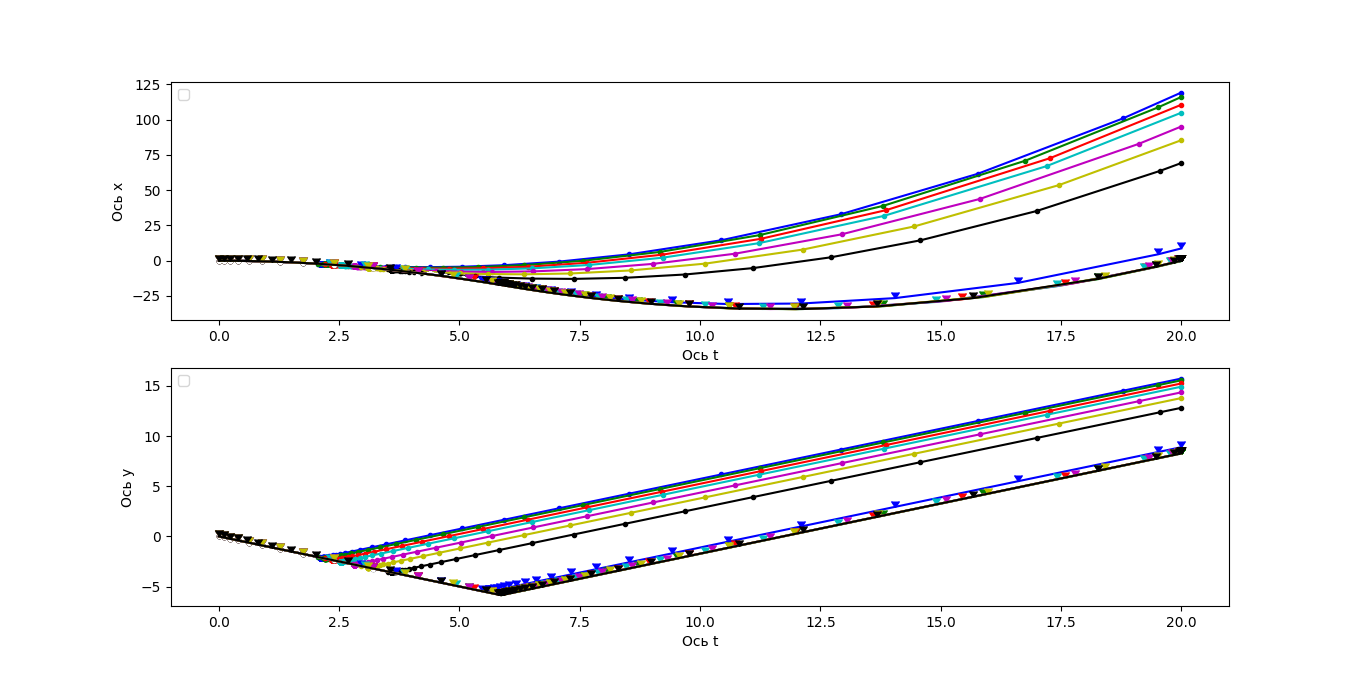
\includegraphics[width=\textwidth, height=12cm]{Figure2_1.png}
\end{figure}
\begin{figure}[H]
    \centering
      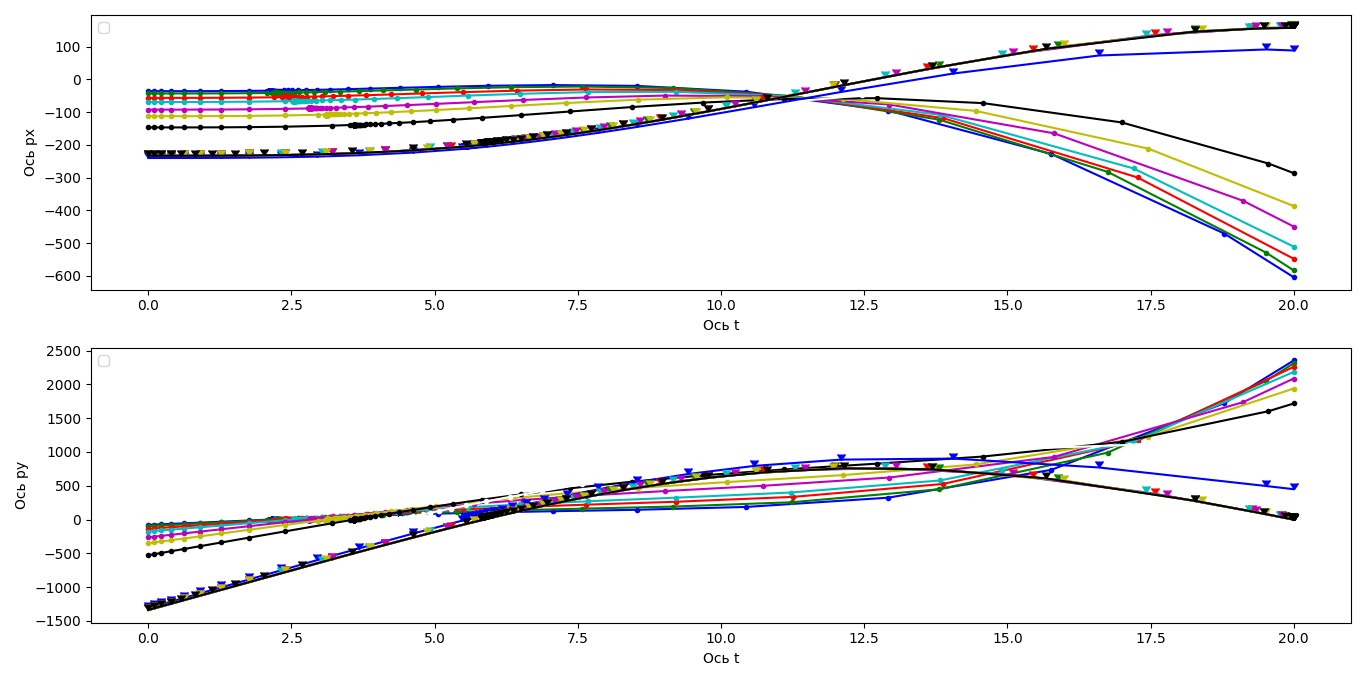
\includegraphics[width=\textwidth, height=12cm]{Figure2_2.png}
\end{figure}
\begin{figure}[H]
    \centering
      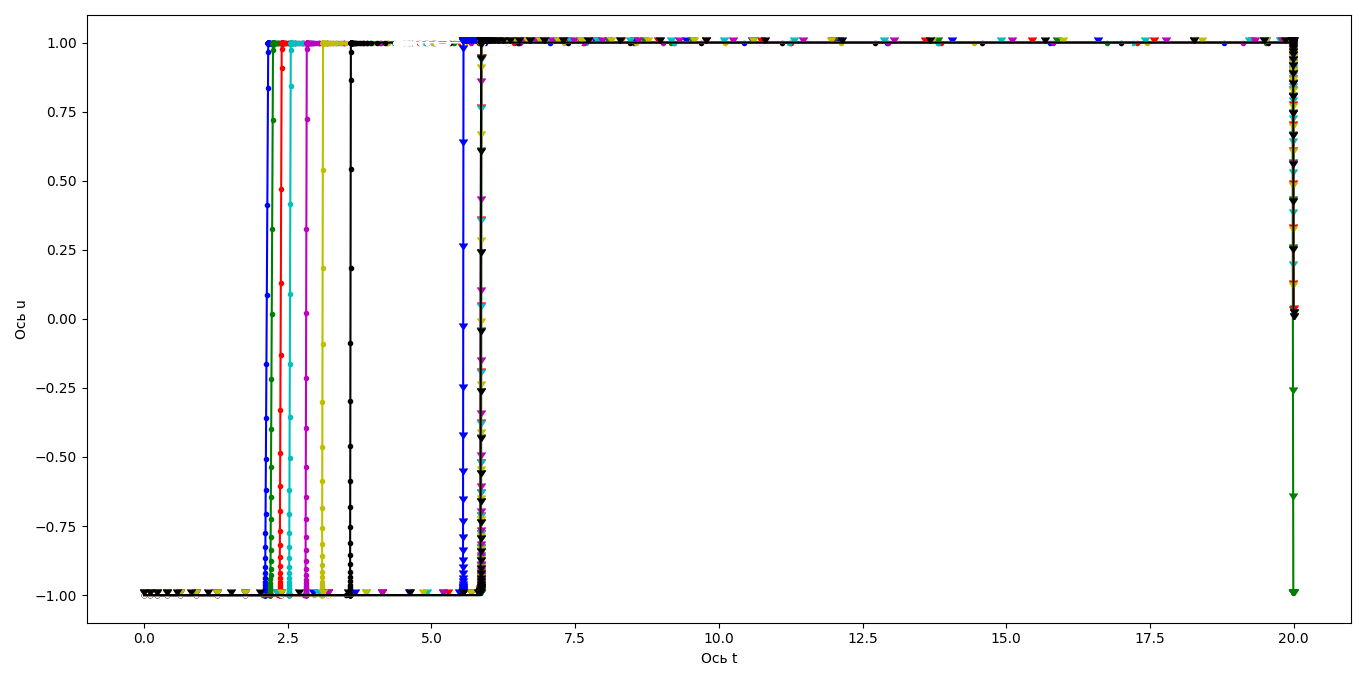
\includegraphics[width=\textwidth, height=10cm]{Figure2_3.png}
\end{figure}
Поэтому теперь нарисуем графики фазовых переменны для финальных параметров пристрелки.
\begin{figure}[H]
    \centering
      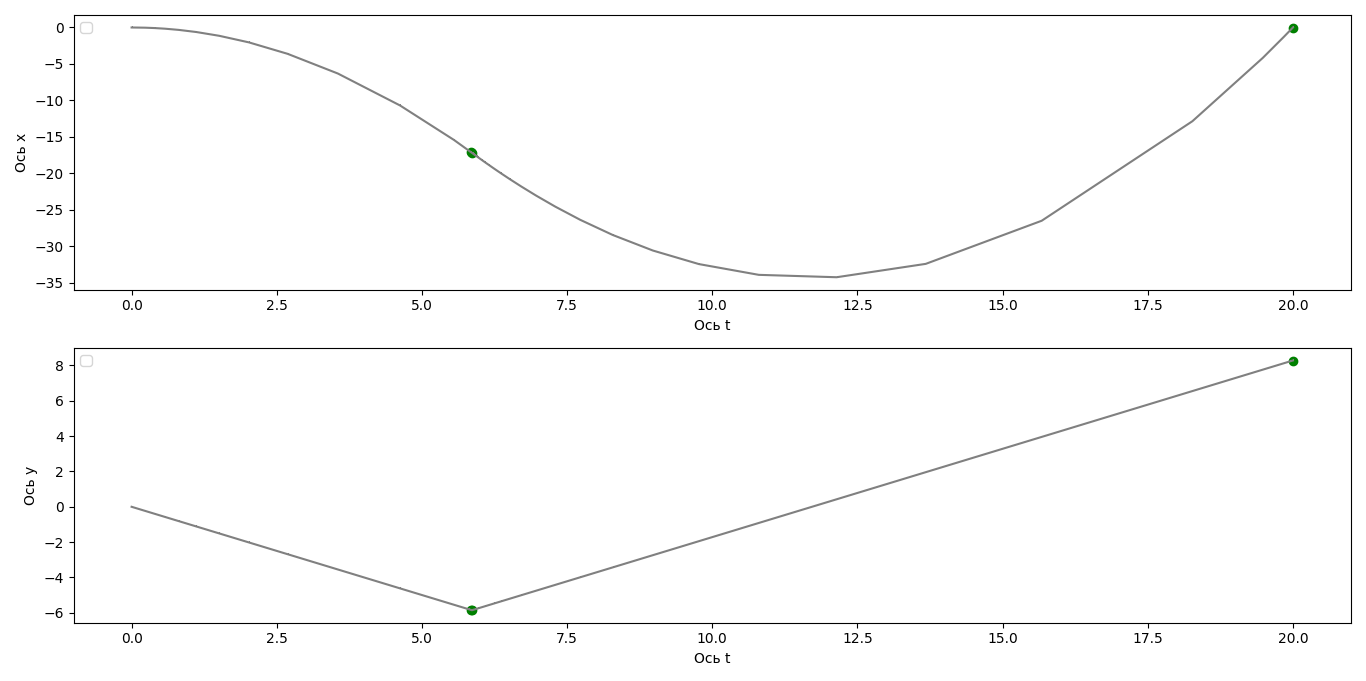
\includegraphics[width=\textwidth, height=12cm]{Figure4_1.png}
\end{figure}
\begin{figure}[H]
    \centering
      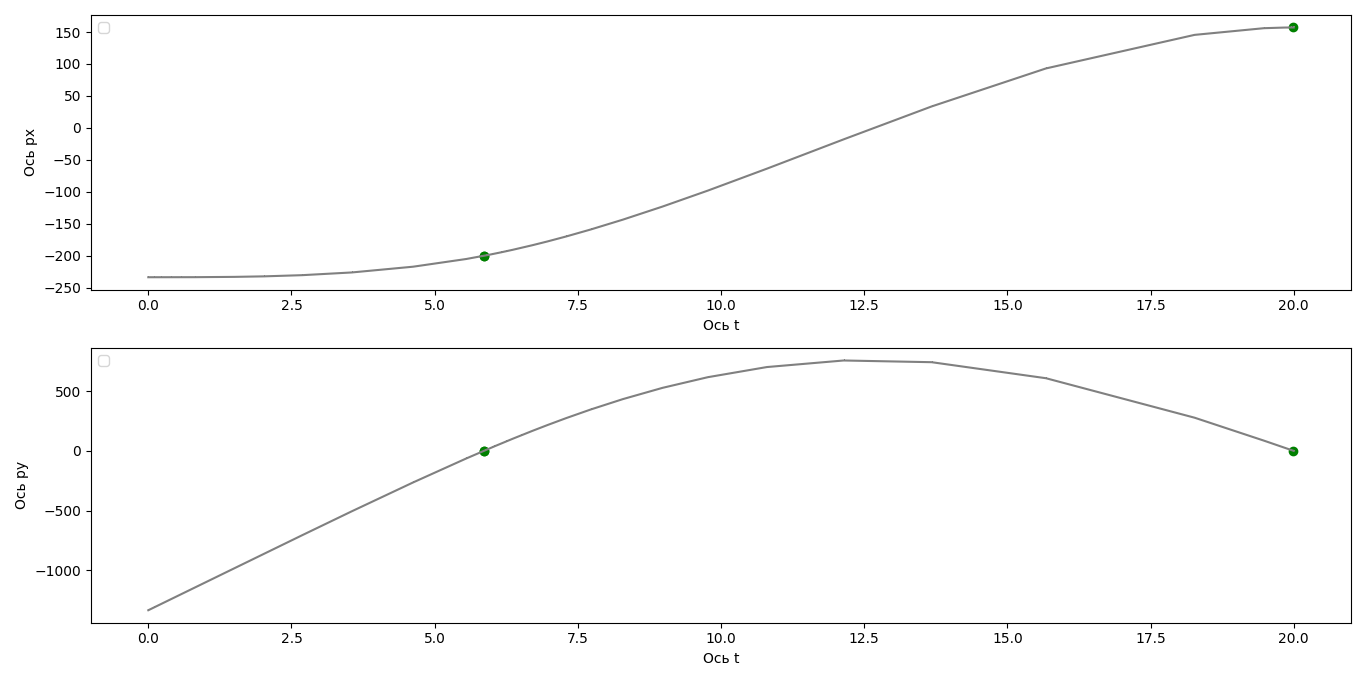
\includegraphics[width=\textwidth, height=12cm]{Figure4_2.png}
\end{figure}
\begin{figure}[H]
    \centering
      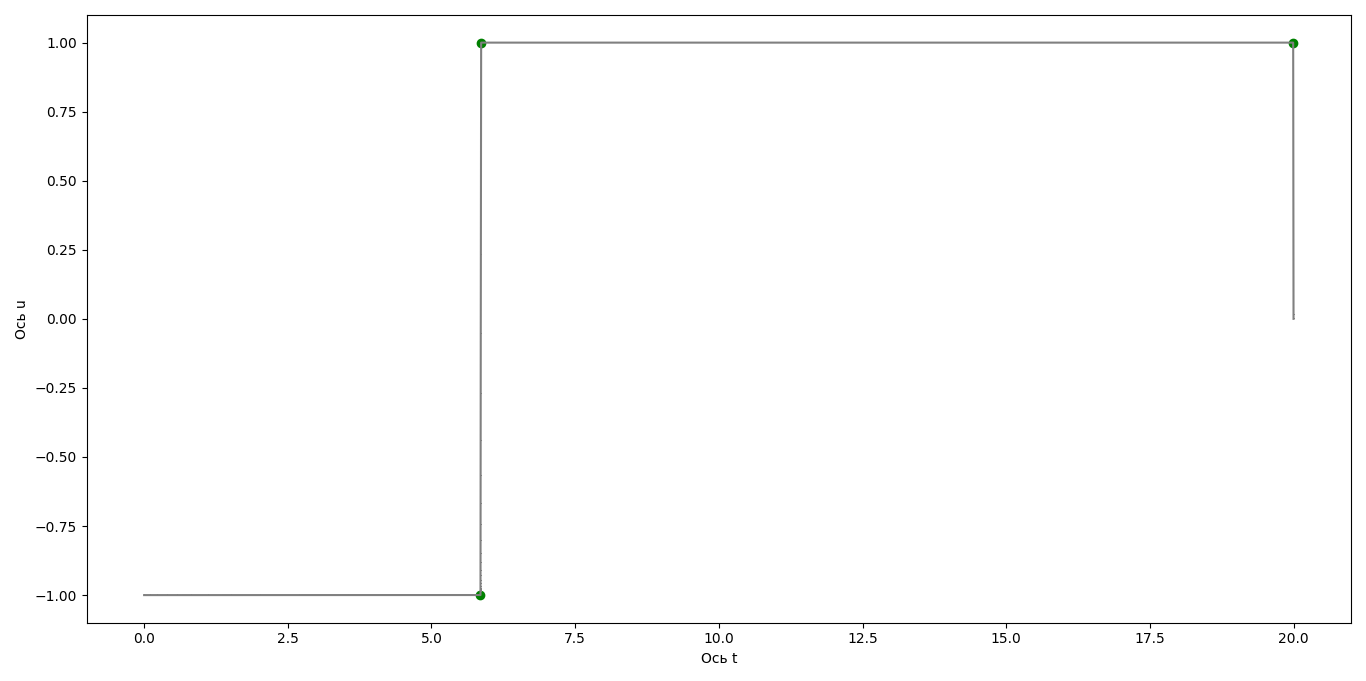
\includegraphics[width=\textwidth, height=6cm]{Figure4_3.png}
\end{figure}
Явно укажим теперь точки переключения для финальных параметров пристрелки.

\begin{center}
\begin{table}[H]
    \begin{tabular}{|c|c|c|c|c|}
        \hline
        $t$&$x(t)$&$y(t)$&$p_x(t)$&$p_y(t)=u$\\
        \hline
        $5.853006$&$-17.12884$&$-5.853006$&$-200.0278$&$-1.00$\\
        \hline
        $5.862724$&$-17.18574$&$-5.853005$&$-199.8611$&$1.00$\\
        \hline
        $19.993953$&$-0.05007457$&$8.278224$&$157.0778$&$1.00$\\
        \hline
    \end{tabular}
\end{table}
\end{center}
Расчет интеграла $B_0=\int_0^T(u^2-y^2-x^2)dt$ дает следующее: $B_0=-10794.147030$ .

Разберемся с случаем T=10. Ниже будут представлены графики, соответсвующие постепенному поиску оптимальной траектории. Эти графики несут лишь изобразительный характер и не содержат самих данных:
\begin{figure}[H]
    \centering
      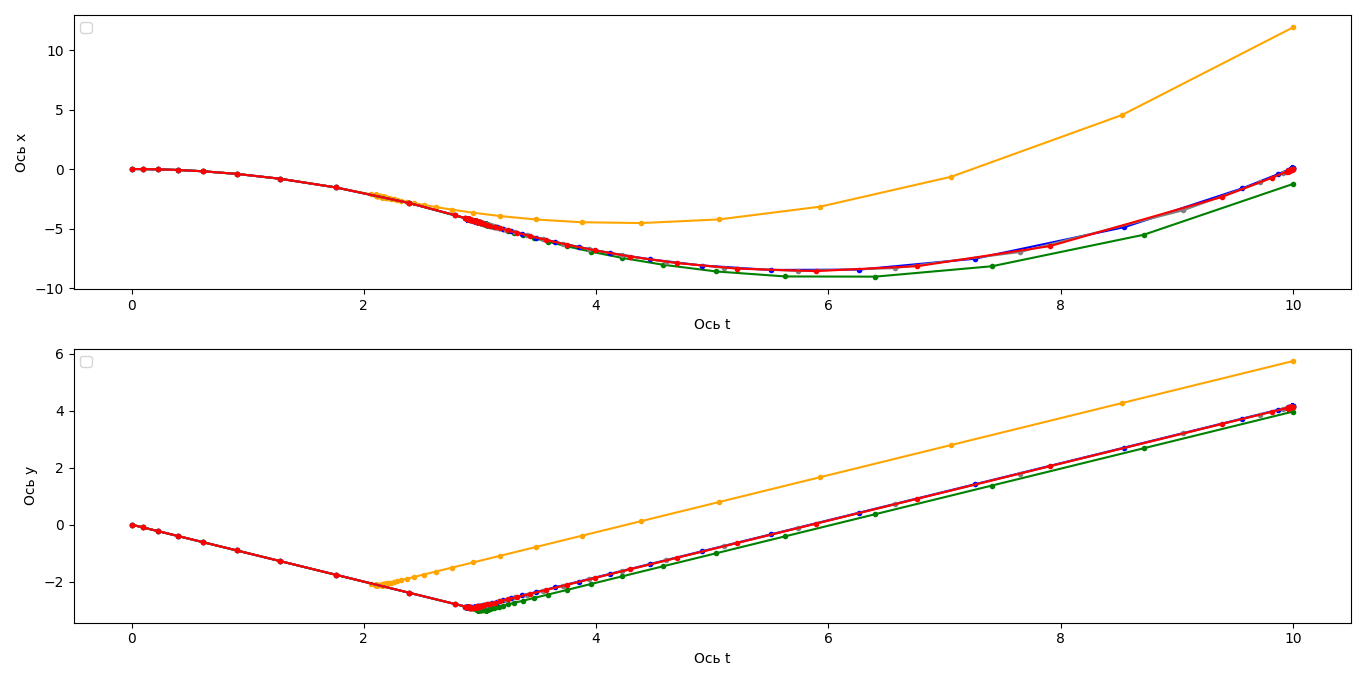
\includegraphics[width=\textwidth, height=12cm]{Figure_1.png}
\end{figure}
\begin{figure}[H]
    \centering
      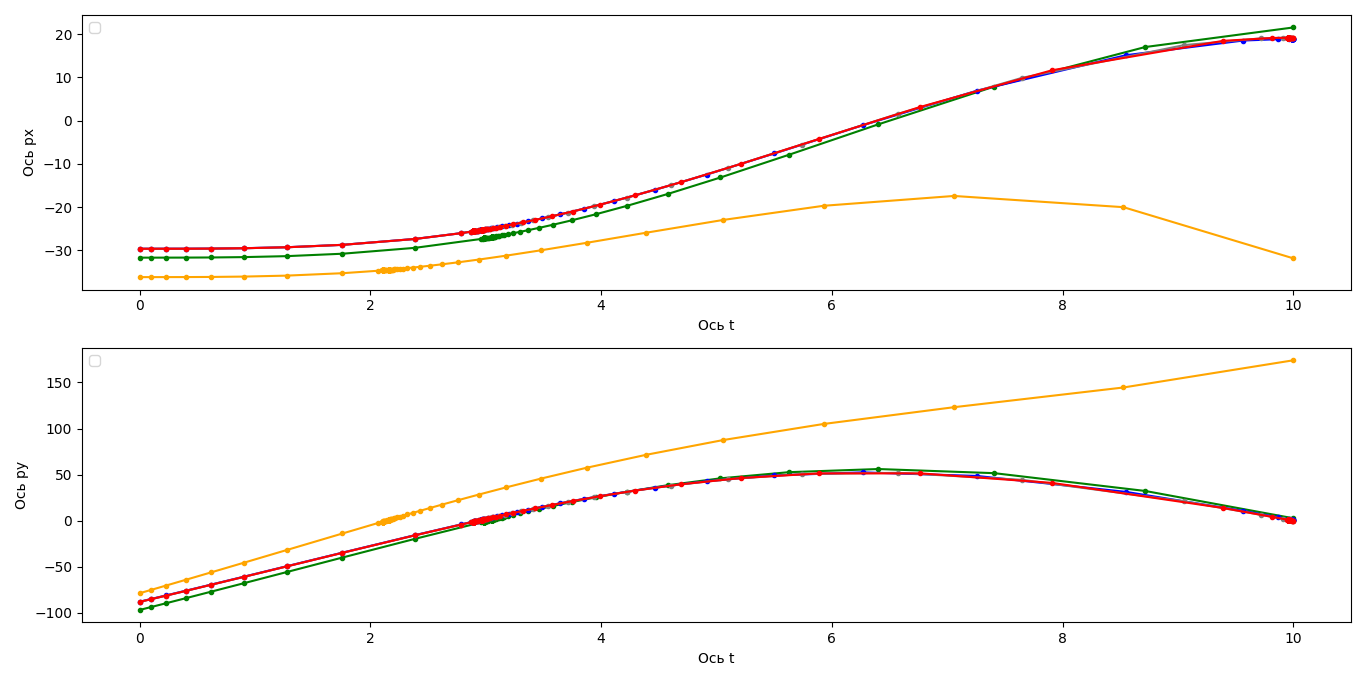
\includegraphics[width=\textwidth, height=12cm]{Figure_2.png}
\end{figure}
\begin{figure}[H]
    \centering
      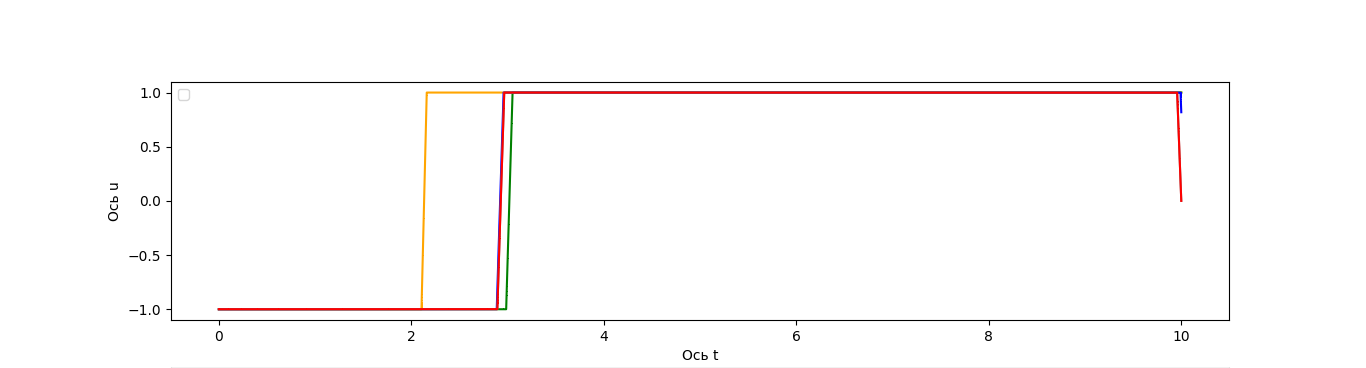
\includegraphics[width=\textwidth, height=10cm]{Figure_3.png}
\end{figure}
Поэтому теперь нарисуем графики фазовых переменны для финальных параметров пристрелки.
\begin{figure}[H]
    \centering
      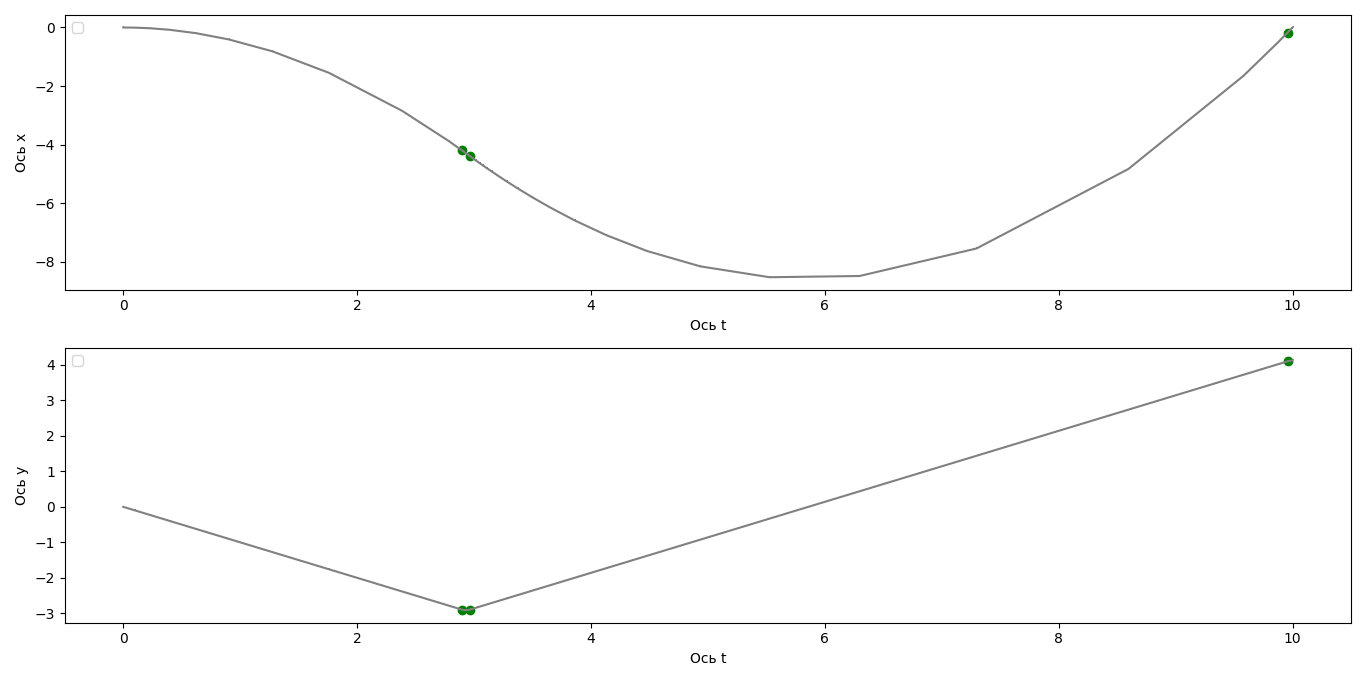
\includegraphics[width=\textwidth, height=12cm]{Figure1_1.png}
\end{figure}
\begin{figure}[H]
    \centering
      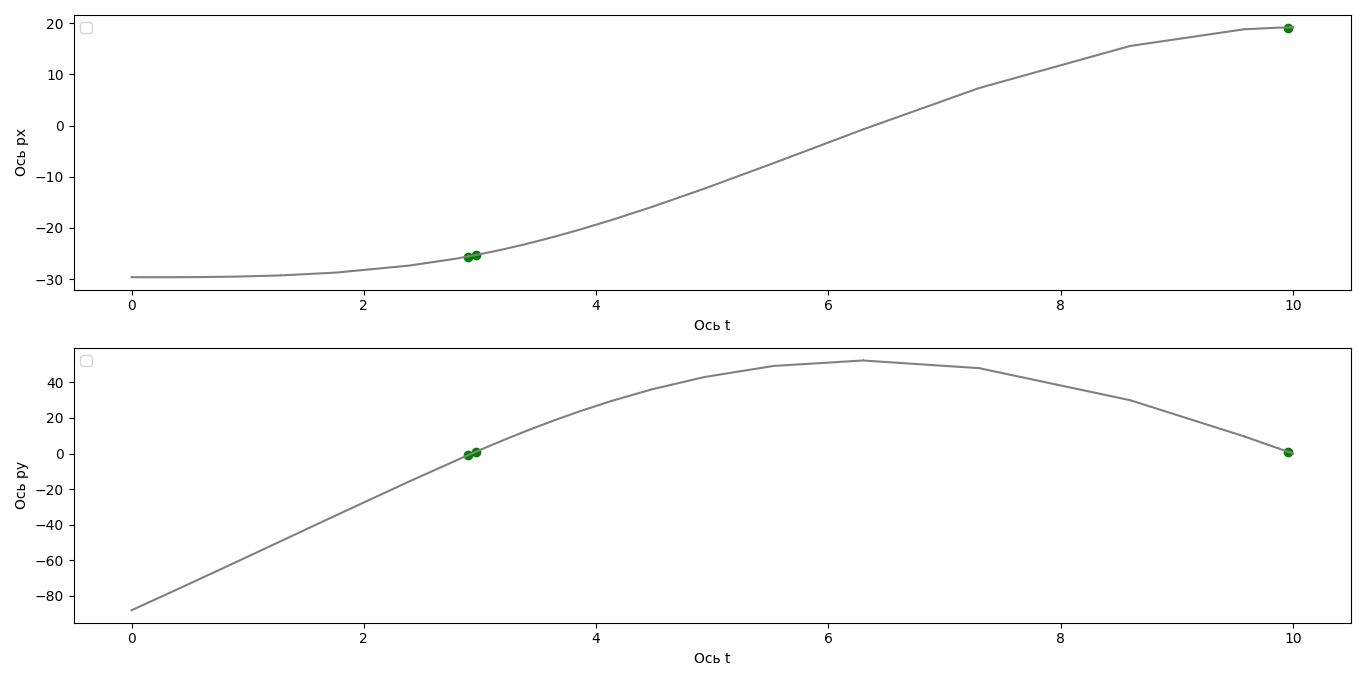
\includegraphics[width=\textwidth, height=12cm]{Figure1_2.png}
\end{figure}
\begin{figure}[H]
    \centering
      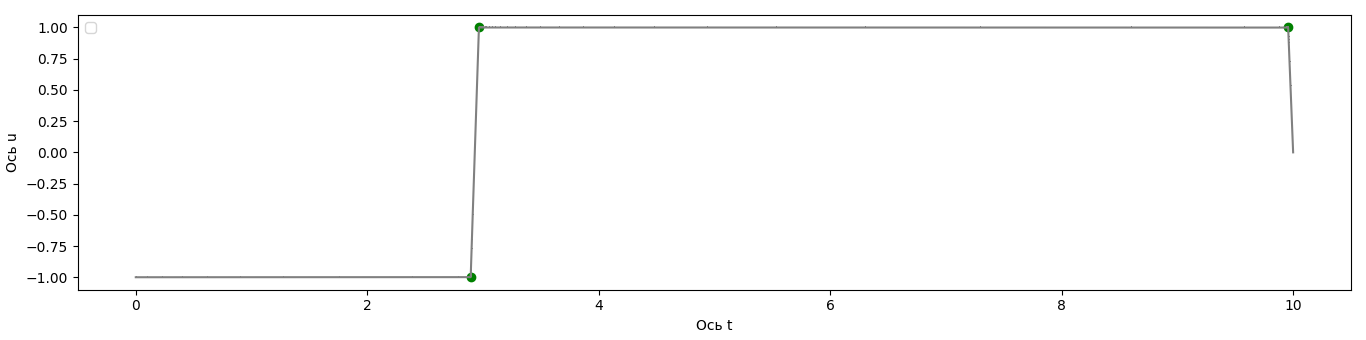
\includegraphics[width=\textwidth, height=6cm]{Figure1_3.png}
\end{figure}
Явно укажим теперь точки переключения для финальных параметров пристрелки.

\begin{center}
\begin{table}[H]
    \begin{tabular}{|c|c|c|c|c|}
        \hline
        $t$&$x(t)$&$y(t)$&$p_x(t)$&$p_y(t)=u$\\
        \hline
        $2.893731$&$-4.186838$&$-2.893731$&$-25.59574$&$-1.00$\\
        \hline
        $2.964275$&$-4.391799$&$-2.893605$&$-25.29316$&$1.00$\\
        \hline
        $9.957065$&$-0.1766136$&$4.099185$&$19.17492$&$1.00$\\
        \hline
    \end{tabular}
\end{table}
\end{center}
Расчет интеграла $B_0=\int_0^T(u^2-y^2-x^2)dt$ дает следующее: $B_0=-358.309826$ .

Что же касается параметров $T=1,T=0.1$ . Будем придерживаться следующей логики, если система состоит из непрерывных функций, то непрерывно изменяя параметр $T$ , то тогда оптимальное решение тоже будет изменяться непрерывно. Поэтому сделаем следующий алгоритм, берем начальные параметры пристрелки при $T=10$ , находим параметры оптимальной траектории, уменьшим $T$ на 0.1, возьмем теперь опять в качестве начальных параметров пристрелки параметры, полученные на предыдущем шаге и повторим алгоритм, и так далее \dots

Таким образом дойдем до того, что при $T=3.3$ - мы можем найти оптимальное управление, но уже при $T=3.2$ - мы уже не можем найти оптимальное управление, поэтому будем считать, что при $T=1, T=0.1$ - нет возможности найти оптимальное решение.

\end{document}
